%%%%%%%%%%%%%%%%%%%%%%%%%%%%%%%%%%%%%%%%%
% University Assignment Title Page 
% LaTeX Template
% Version 1.0 (27/12/12)
%
% This template has been downloaded from:
% http://www.LaTeXTemplates.com
%
% Original author:
% WikiBooks (http://en.wikibooks.org/wiki/LaTeX/Title_Creation)
%
% License:
% CC BY-NC-SA 3.0 (http://creativecommons.org/licenses/by-nc-sa/3.0/)
% 
% Instructions for using this template:
% This title page is capable of being compiled as is. This is not useful for 
% including it in another document. To do this, you have two options: 
%
% 1) Copy/paste everything between \begin{document} and \end{document} 
% starting at \begin{titlepage} and paste this into another LaTeX file where you 
% want your title page.
% OR
% 2) Remove everything outside the \begin{titlepage} and \end{titlepage} and 
% move this file to the same directory as the LaTeX file you wish to add it to. 
% Then add \input{./title_page_1.tex} to your LaTeX file where you want your
% title page.
%
%%%%%%%%%%%%%%%%%%%%%%%%%%%%%%%%%%%%%%%%%
%\title{Title page with logo}
%----------------------------------------------------------------------------------------
%    PACKAGES AND OTHER DOCUMENT CONFIGURATIONS
%----------------------------------------------------------------------------------------

\documentclass[12pt]{article}
\usepackage[english]{babel}
\usepackage[utf8x]{inputenc}
\usepackage{amsmath}
\usepackage{graphicx}
\usepackage[colorinlistoftodos]{todonotes}

\begin{document}

\begin{titlepage}

\newcommand{\HRule}{\rule{\linewidth}{0.5mm}} % Defines a new command for the horizontal lines, change thickness here

\center % Center everything on the page
 
%----------------------------------------------------------------------------------------
%    HEADING SECTIONS
%----------------------------------------------------------------------------------------

\textsc{\LARGE Kyung Hee University}\\[1.5cm] % Name of your university/college
\textsc{\Large School of Electronics and Information}\\[0.5cm] % Major heading such as course name
\textsc{\large Department of Computer Engineering}\\[0.5cm] % Minor heading such as course title

%----------------------------------------------------------------------------------------
%    TITLE SECTION
%----------------------------------------------------------------------------------------

\HRule \\[0.4cm]
{ \huge \bfseries IBM Internet of Things: Turn your mobile device into a sensor}\\[0.4cm] % Title of your document
\HRule \\[1.5cm]
 
%----------------------------------------------------------------------------------------
%    AUTHOR SECTION
%----------------------------------------------------------------------------------------

\begin{minipage}{0.45\textwidth}
\begin{flushleft} \large
\emph{Author:}\\
Le Pham \textsc{Tuyen} (2014311082) \\
Nguyen Thi My \textsc{Kieu} (2014311076)
\end{flushleft}
\end{minipage}
~
\begin{minipage}{0.45\textwidth}
\begin{flushright} \large
\emph{Supervisor:} \\
Professor \textsc{Choong Seon Hong} % Supervisor's Name
\end{flushright}
\end{minipage}\\[2cm]

%----------------------------------------------------------------------------------------
%    DATE SECTION
%----------------------------------------------------------------------------------------

{\large \today}\\[0cm] % Date, change the \today to a set date if you want to be precise

%----------------------------------------------------------------------------------------
%    LOGO SECTION
%----------------------------------------------------------------------------------------


\includegraphics[width=0.25\textwidth]{logo.png}\\[1cm] % Include a department/university logo - this will require the graphicx package
 
%----------------------------------------------------------------------------------------

\vfill % Fill the rest of the page with whitespace

\end{titlepage}


\begin{abstract}

The Internet of Things (IoT) is a significant trend of the future internet. It is a computing concept that describes a future where daily physical objects will be connected to the internet and be able to identify themselves to other devices. The potential IoT application areas are smart cities (and regions), smart car and mobility, smart home and assisted living, smart industries, public safety, energy $\&$ environmental protection, agriculture, and tourism. So far, the IoT continues to affirm its important position in the context of information and communication technologies, and the development of society. Our report will introduce the newest technology of IBM in IoT. Particularly, we will introduce an application, called Health Monitoring, use MQTT protocol of IBM.

\end{abstract}

\section{Introduction}

\begin{figure*}[htbp]
\centering
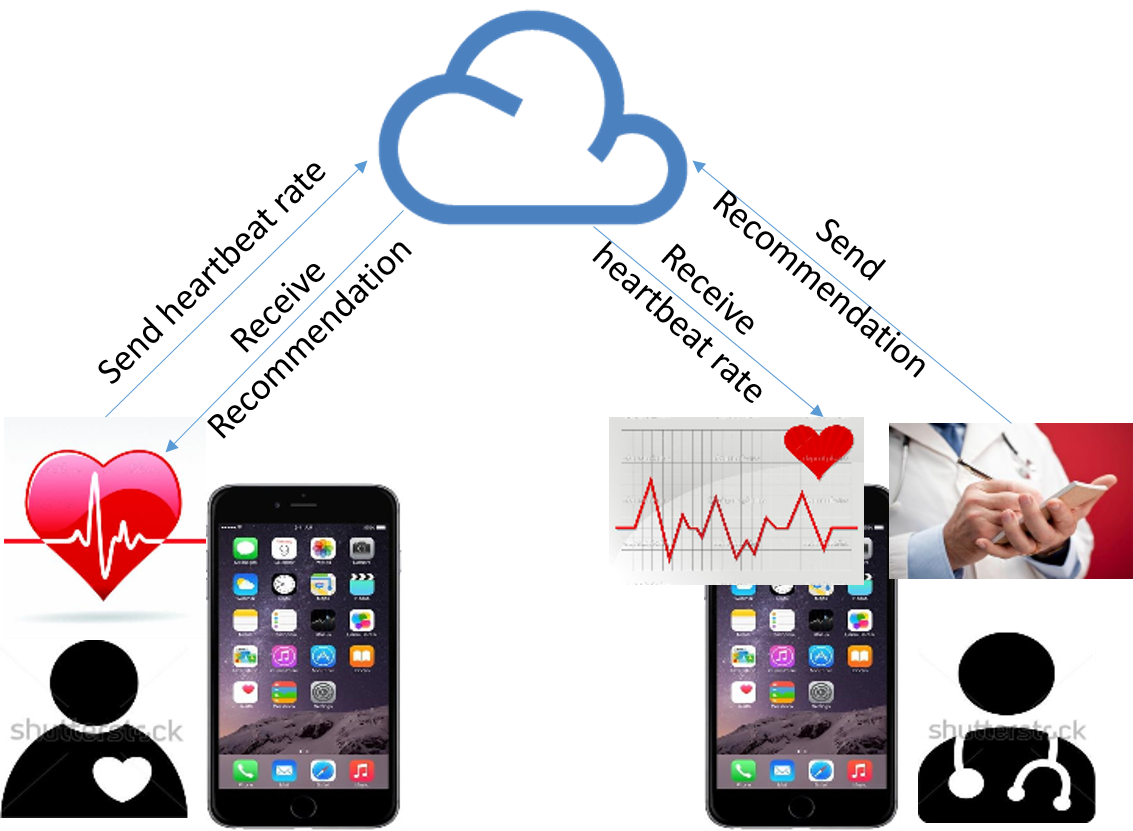
\includegraphics[width=0.75\textwidth]{scenario1.png}
\caption{Measuring the heartbeat rate and send it to doctor}
\label{fig:scenario1}
\end{figure*}

Nowadays, smartphones have become popular, powerful, cheap and able to connect the internet anytime, anywhere. Besides that, it contains so many sensors, such as camera sensor, gyro sensor, GPS sensor, and we can use these sensors to turn your smartphone into a part of IoT scenarios. Our project focuses on healthcare scenarios using smartphones. We developed two application on iPhone device, one for the patient and one for the doctor. The patient uses our application to measure the heartbeat rate and sends it to the doctor. The application on doctor's iPhone will visualize the heartbeat rate in a graph. After that, the doctor can send back the recommendation to the patient.

In addition, if the patient is in an emergency situation and needs a support from the doctor, he can make an emergency call to the doctor. Immediately, a warning message will show up on the doctor's iPhone combined with alert sound. After receiving the warning message, the doctor can quickly come to the patient's location. Our application allows the doctor to monitor the patient's location and show that location on the map.

\begin{figure*}[htbp]
\centering
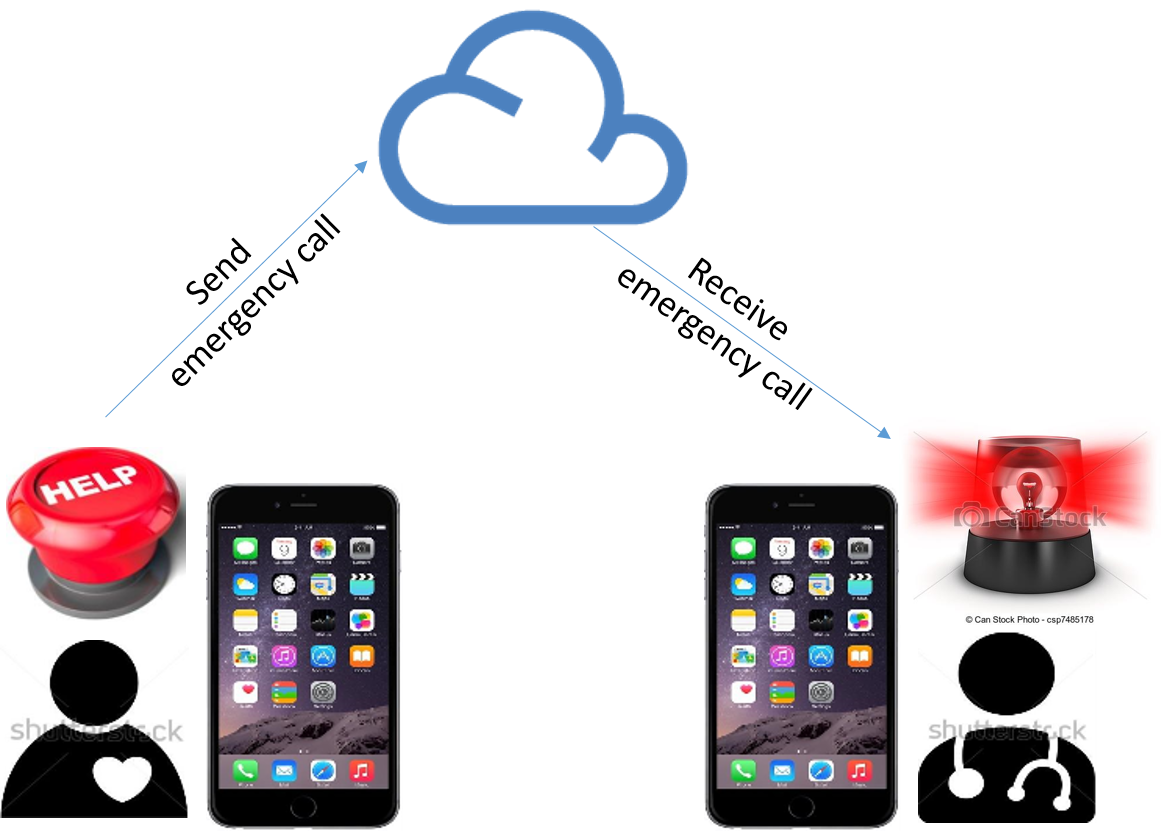
\includegraphics[width=0.75\textwidth]{scenario2.png}
\caption{The patient make an emergency call to the doctor}
\label{fig:scenario2}
\end{figure*}

\begin{figure*}[htbp]
\centering
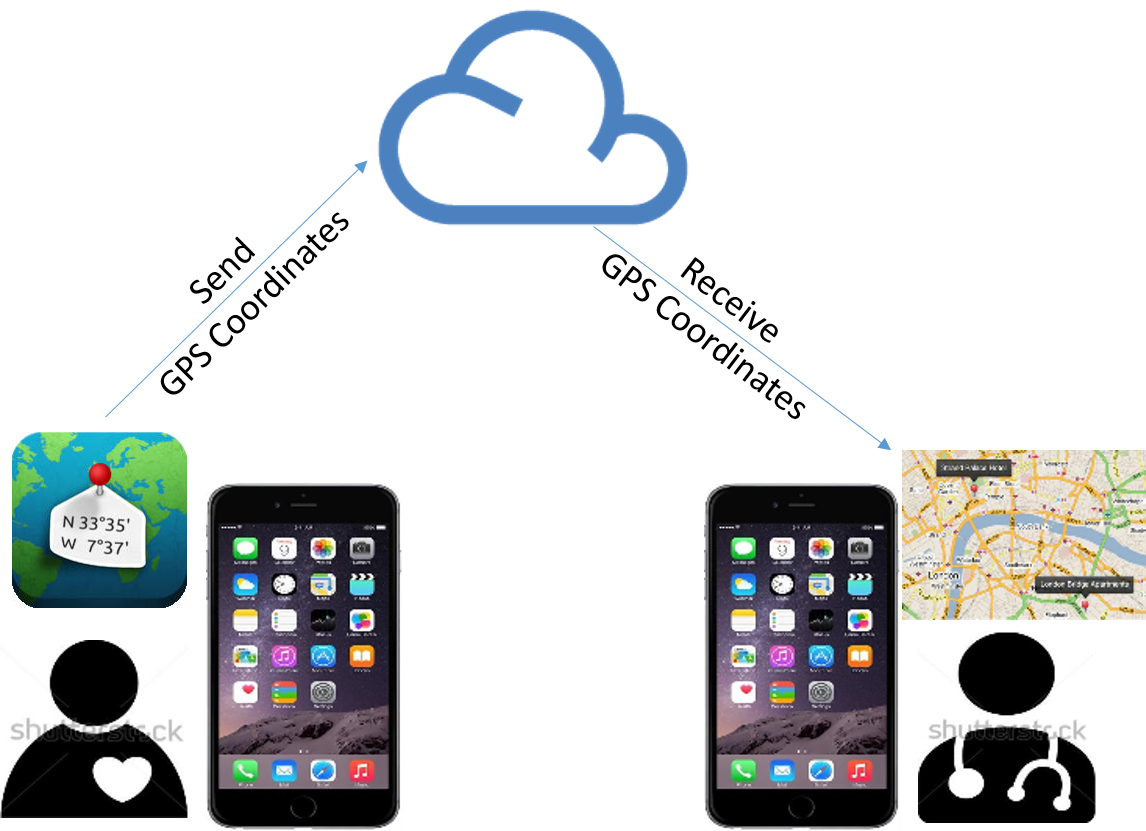
\includegraphics[width=0.75\textwidth]{scenario3.png}
\caption{The doctor monitors the patient's location}
\label{fig:scenario3}
\end{figure*}

In order to make the application with the features mentioned above, we need an IoT framework meet following requirements. Firstly, the framework allows a device to send the data to many devices. In our case, the patient can send heartbeat rate or make an emergency call to many doctors. Secondly, the IoT framework needs to provide the real-time application. The device can receive the data immediately after the sender sent the data. Thirdly, The IoT framework minimizes the sending packets of data. Finally, The IoT framework needs to provide reliably pushing data over an unreliable network. Besides that, they should have the requirements such as saving power consumption, security, and scalability... MQTT protocol is designed to meet these requirements and we selected it to make our application.

\section{MQTT Protocol}

MQTT is a machine-to-machine (M2M)/"Internet of Things" connectivity protocol. It was designed as an extremely lightweight publish/subscribe messaging transport. MQTT was invented by Dr. Andy Stanford-Clark of IBM, and Arlen Nipper of Arcom (now Eurotech), in 1999. It's open and you can visit the website MQTT.org to see the specification and standard. It is easy to use MQTT Protocol because it only supports a small number of APIs such as connecting and disconnecting the server, publishing and subscribing a topic. MQTT was designed for minimizing the sending packet by reducing the header size or using the binary payload. Depending on your purpose, MQTT provides the options to control the QoS for message delivery. MQTT supports client libraries for Java, C, and Javascript. So, you can easily develop your application on Android, iOS, and web-based application.

\begin{figure*}[htbp]
\centering
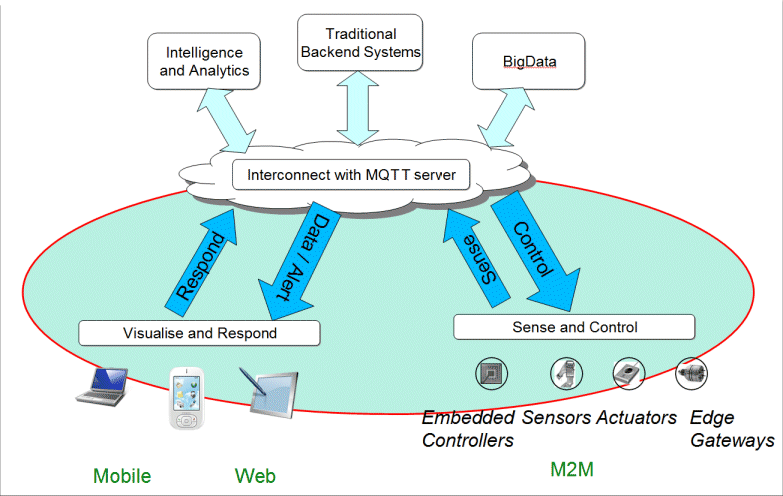
\includegraphics[width=0.75\textwidth]{mqtt.png}
\caption{MQTT Protocol}
\label{fig:mqtt}
\end{figure*}

\section{iPhone Application: Health monitoring}

\begin{figure*}[htbp]
\centering
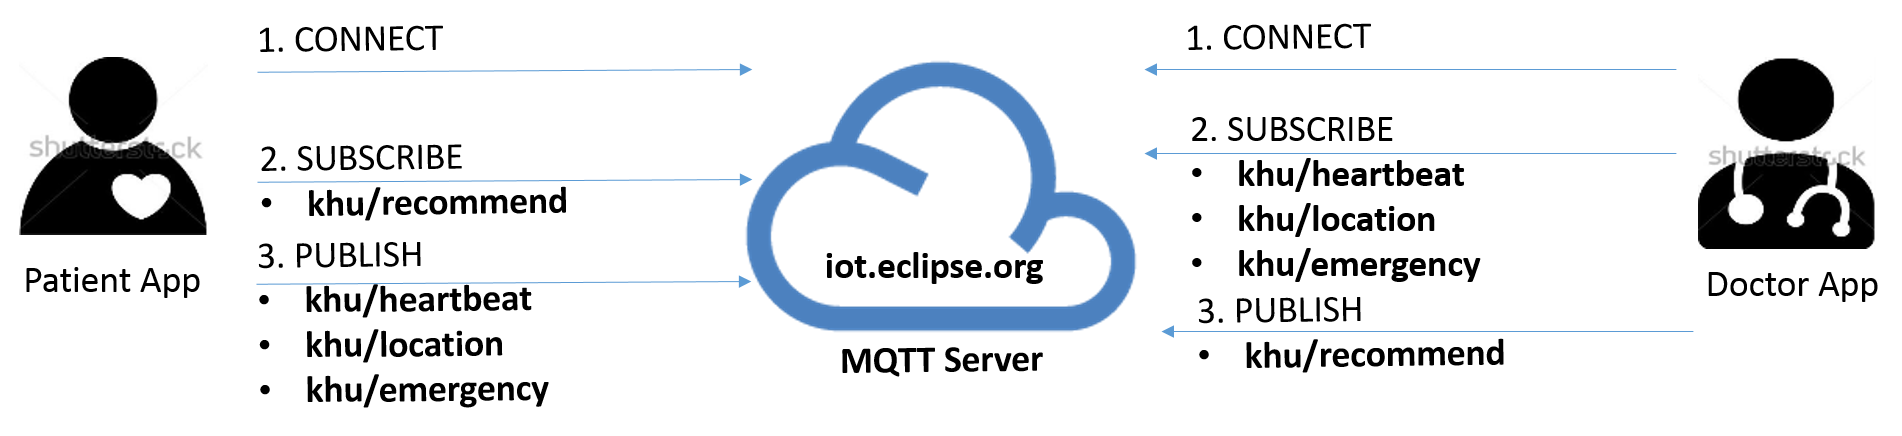
\includegraphics[width=1\textwidth]{design.png}
\caption{Work flow of our application}
\label{fig:design}
\end{figure*}

After selecting the MQTT protocol for our application, we develop a couple of applications on iPhone, one for the patient and one for the doctor. Besides that, we have a MQTT server in the middle to receive and forward messages between sender and receiver. In case of patient application, The patient needs to connect the application to the server before using it. After connected to the server, it must subscribe the topic \textbf{khu$/$recommend}. This step allows the patient's application to receive recommendation message from the doctor. Finally, the patient's application will publish the data combined with a specified topic. In this case, the patient application will publish with one of three topics: \textbf{khu$/$heartbeat}, \textbf{khu$/$location}, \textbf{khu$/$emergency}. Similarly, the doctor's application also follows the same steps as the patient's application. It subscribes the topics sent from the patients and publishes the topic received from patients.

The demo of applications is running on iPhone 5s. The detailed flow of applications is shown in Figure \ref{fig:patient} and Figure \ref{fig:doctor}. The interesting thing is that you can measure the heartbeat rate using iPhone. Basically, your skin color related to heartbeat rate. So, the algorithm might capture the changes from skin color and transform to heartbeat rate. The technical detail behind them please read the paper \cite{Poh}

\begin{figure*}[htbp]
\centering
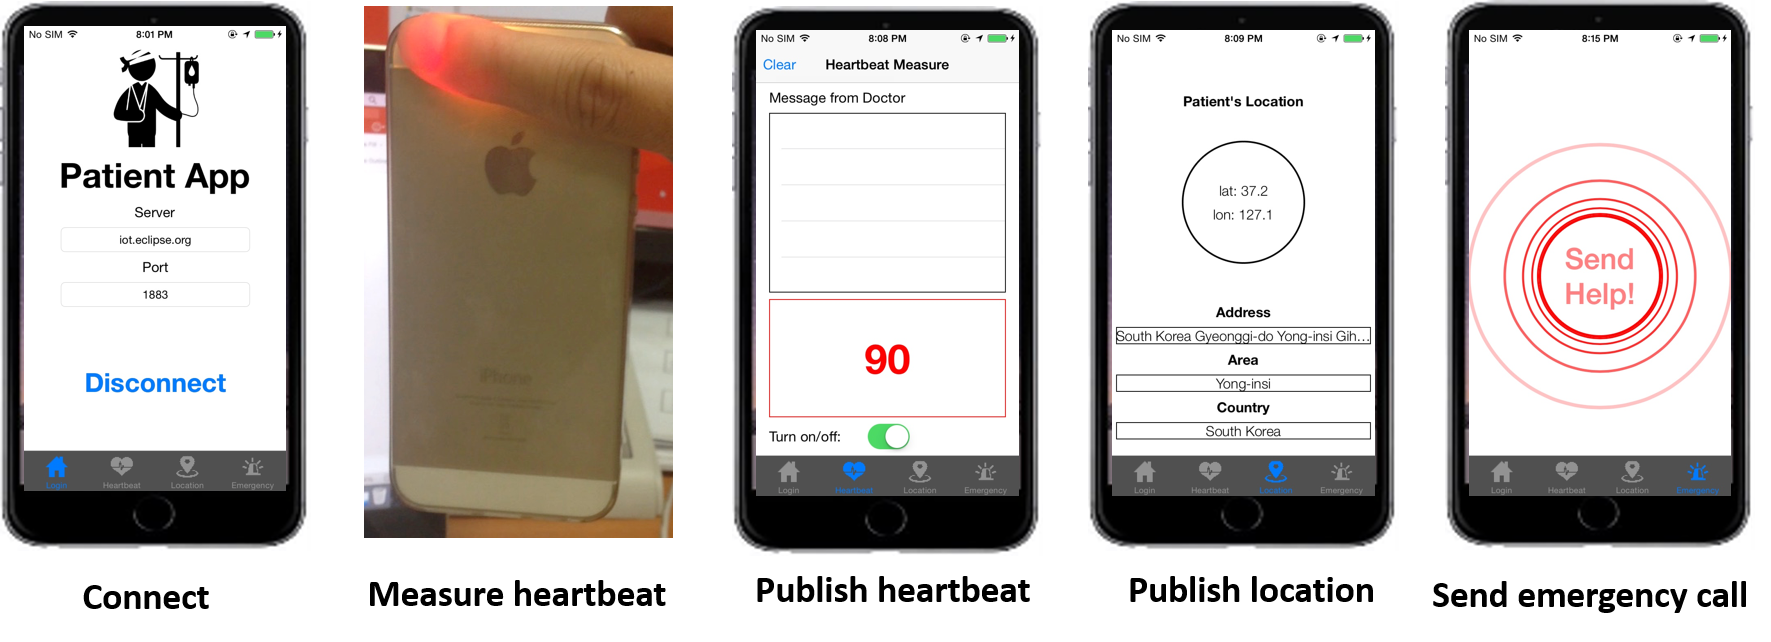
\includegraphics[width=1\textwidth]{patient.png}
\caption{Work flow of patient application}
\label{fig:patient}
\end{figure*}

\begin{figure*}[htbp]
\centering
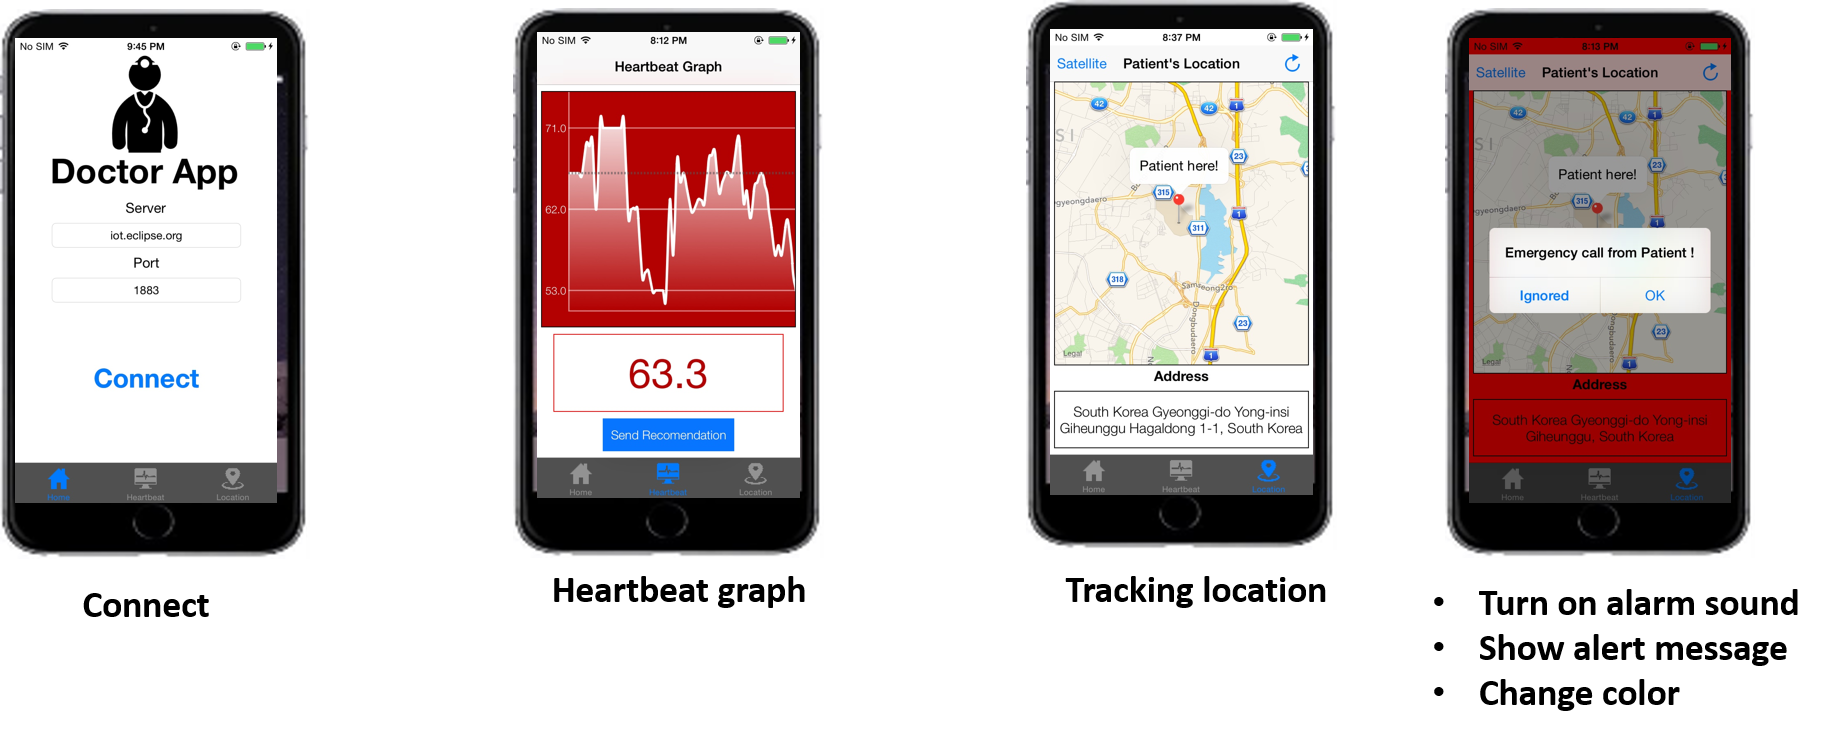
\includegraphics[width=1\textwidth]{doctor.png}
\caption{Work flow of doctor application}
\label{fig:doctor}
\end{figure*}

\section{Conclusion}

Our project introduced to you an IoT protocol of IBM. Through this protocol, IBM provides a service allowing a billion of devices to connect together. Besides, many creative IoT applications can be deployed quickly based on this protocol. Although our application is a simple example of IoT application, it has the potential to expand to a business to provide customers such as doctor, patient...

\begin{thebibliography}{99}

\bibitem{IBMIoT} 
IBM Internet of Things Foundation,
\\\texttt{https://internetofthings.ibmcloud.com/}

\bibitem{MQTT} 
MQTT Protocol,
\\\texttt{http://mqtt.org/}

\bibitem{SourceCode} 
Source code of Health Monitoring,
\\\texttt{https://github.com/lephamtuyen/healthmonitoring}

\bibitem{Poh} Poh, Ming-Zher, Daniel J. McDuff, and Rosalind W. Picard. \emph{"Non-contact, automated cardiac pulse measurements using video imaging and blind source separation."} Optics express 18.10 (2010): 10762-10774.

\end{thebibliography}

\end{document}